\input{../tikz-header}
\begin{document}
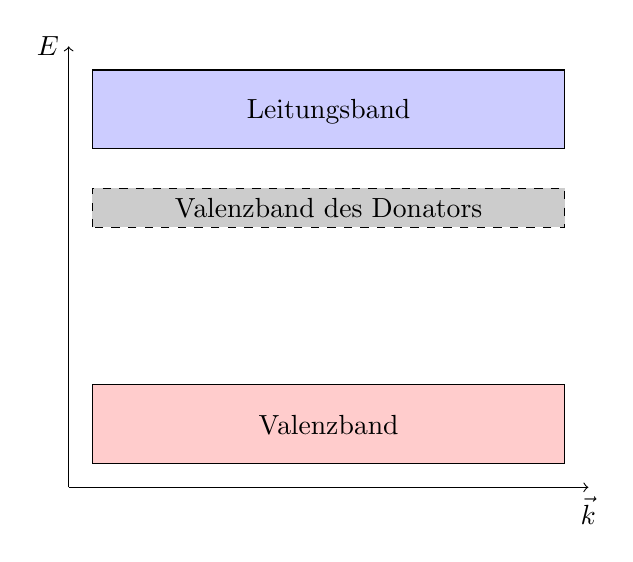
\begin{tikzpicture}
    \draw[fill=red, fill opacity=0.2] (0,0) rectangle (6,1);
    \node[above, yshift=0.25cm] at (3,0) {Valenzband};

    \draw[fill=blue, fill opacity=0.2] (0,4) rectangle (6,5);
    \node[below, yshift=-0.25cm] at (3,5) {Leitungsband};

    % \draw[->] (1,3.5) -- (1,4);
    % \draw[->] (0.3,1) -- (0.3,4);
    % \draw[<-] (0.6,1) -- (0.6,4);

    \draw[dashed,fill=black, fill opacity=0.2] (0,3) rectangle (6,3.5);
    \node[below, yshift=0.5cm] at (3,3) {Valenzband des Donators};

    \draw[->] (-0.3,-0.3) -- (-0.3, 5.3) node[left]{$E$};
    \draw[->] (-0.3,-0.3) -- (6.3,-0.3) node[below]{$\lvert\vec{k}\rvert$};
\end{tikzpicture}
\end{document}